\chapter{Technologie wykorzystane w aplikacji}
Poniższy rozdział opisuje opsuje wewnętrzną architekturę aplikacji. Zwraca uwagę na jej wielowarstwowy charackter. Dla każdej z warstw opsisuje technologie w których dana warstwa może być realizowana zwracając szczególną uwagę na te, które zostały wybrane do jej faktycznej implementacji.

\section[Aplikacja w architekturze wielowarstwowej][Aplikacja w architekturze wielowarstwowej]{Aplikacja w architekturze wielowarstwowej}
Podział systemu na warstwy pozwala na ułatwienia w całym cyklu życia aplikacji. W szczególności zmniejsza koszty jego modyfikacji, gdyż wpowadzane zmiany agraniczają się zazwyczaj tylko do jednej warstwy. 

Najprostrzym przykładem wielowarswowej architektury aplikacji jest model typu klient-serwer. Wyróżnia on dwie warstwy:
\begin{itemize}
	\item klienta, stronę żądającą dostępu do jakiejś usługi bądź zasobu,
	\item serwera, stronę udostępniająca daną usługę lub zasób.
\end{itemize}
Architektura ta dobrze sprawdzająca w małych systemach zaczęła sprawiać problemy wraz z rozrostaniem się logik biznesowych aplikacji. Efektem tego było pojawienie się pojeć cieknkiego i grubego klienta(ang. \textit{thin client} i \textit{fat client}) dla określnia technik umieszających logikę biznesową po jednej lub po drugiej stronie.

Ostatecznie projektanci systemów wydzielili jeszcze jedną warstwę(odpowiedzialną za realizcję logiki biznesowej) dporowadzając do powstania architektury trójwarswowej. Wyróżnia ona następujące warstwy:
\begin{itemize}
	\item warstwę prezentacji widoczną dla kielnta,
	\item warstwę aplikacji ralizującą logike biznesową,
	\item warstwę źródła danych.
\end{itemize}
Rysunek \ref{warstwy} przestawia ogólny schemat aplikacji trójwarstowej.

\begin{figure}[tdh]
    \begin{center}
	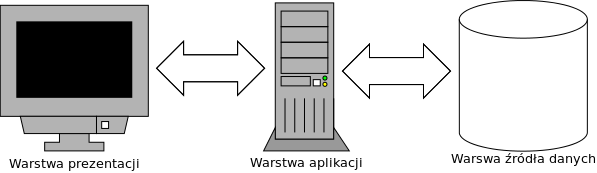
\includegraphics[scale=.7 ]{img/warstwy.png}
	\caption{Schemat komunikacji w architekturze trójwarstwowej}
	\label{warstwy}
    \end{center}
\end{figure}


\section[Warstwa prezentacji][Warstwa prezentacji]{Warstwa prezentacji}
Warstwa prezentacji stanowi interfejs miedzy użytkownikiem a systemem. Najbardziej podstawową implementacją tej warswy jest terminal znakowy. Funkcje taką może pełnić również aplikacja okienkowa. W przypadku aplikacji webowych(takich jak ta) warstwa ta jest realizowana w przeglądarce internetowej za pomocą typowych technologii(takich jak HTML, CSS czy JavaScript).

\subsection[HTML][HTML]{HTML}
Podstawową technologią wyjorzystywaną do tworzenia widoków aplikacji internetowych jest język znaczników HTML(ang. \textit{Hypertext Markup Language}). Najważniejszą jego zaletą jest przenośność. Zyskujemy dzięki temu niezależność interfejsu od środowiska użytkownika. Niestety sposób prezentacji wciąż zależy jednak(w niewielkim stopniu) od przeglądarki, więc jednym z etapów projektu powinno być zawsze założenie jakie przeglądarki i od jakiej wersji będą przez nas wspieranie. Należy też pamiętąć że standard HTML również podlega wersjonowaniu, co oznacza konieczność upewnienia się wpierana przez nas przeglądrka obsługuje HTML w jego najnowszej - piętej wersji. W przeciwnym wypdadku musimy ograniczyć się do funkcjonalności z wersji wcześniejszych.

Kolejną zaletą języka znaczników jest jego prostota, dzięki której nawet początkujący web-designerzy są w stanie szybko nauczyć się pisania kodu HTML.

Wadą języka HTML jest jego statyczność, nawet najmniejsza zmiana na stronie wymaga ponownego wygenerowania żądania HTTP i przesłania go do serwera. Wpływa to negatywnie na responsywność aplikacji, szczególnie przy dużym obciążeniu. 
%Zdanie z SDI troche bez sensu ale mozna podrasowac
%Rozwiązaniem tego problemu są technologie takie jak np. AJAX, które generują kod wykonywany na poziomie przeglądarki, bez konieczności ponownego przesyłania żądania.

\subsection[CSS][CSS]{CSS}
W języku HTML możliwe jest wskazanie sposobu wyświetlania informacji, zaleca się jednak aby treść dokumentu była odseparowana od sposobu jej prezentacji. Umożliwiają to kaskadowe arkusze stylów(CCS). Pozwalają one wydzielenie opisu sposobu prezentacji do specjalnych plików. Zastsowwanie tzw. selektorów możliwe jest zdefiniowanie jednolitego stylu dla całej aplikacji. Łatwiejsze staje się też zarządzanie jej wyglądem.

\subsection[JavaScript][JavaScript]{JavaScript}
JavaScript jest językiem skryptowym wykonywanym po stronie przeglądarki. Pozwala na cześciowe ominięcie problemu statyczności dokumentu HTML. Zastosowanie JavaScriptu pozwala osiągnąc większą responsywność stron internetowych. Do typowych jego zastosowań należy obsługa dynamicznych elementów aplikacji (takich jak okna dialogowe) czy wstępna walidacja formularzy. Za pomocą JavaScriptu możemy też manipulować drzewem DOM dokumentu HTML.

\subsection[AJAX][AJAX]{AJAX}
AJAX(ang. \textit{Asynchronous JavaScript and XML}) jest to wieloelemntowa technologia pozwalająca na twierzenie kodu wykonującego się w całości po stronie klienta bez konieczmności przeładowywania stron. Daje ona możliwość wysyłania asynchronicznych zapytań do serwera. Pozwala to rozwiązać problem statyczności kodu HTML i daje możliwość tworzenia stron w pełni dynamicznych. Rozwiązanie to ma jednakt też kilka wad:
\begin{itemize}
	\item utrudnione zarządzanie historią w przeglądarce(mechanizmy pozwalające rozwiązać ten problem pojawiły dopiero w HTML5),
	\item długi czas ładowania aplikacji(szczególnie w przypadku wolnych łącz).
\end{itemize}
Oprócz wposmnianych wcześniej HTML'a, CSS'a i JavaScriptu w sład technologii AJAX wchodzą również:
\begin{itemize}
	\item XMLHttpRequest, klasa umożliwiająca asynchroniczne przesyłanie danych,
	\item XML(ang. \textit{Extensible Markup Language}), język znaczników pozwalający na przesyłanie informacji między klientem a serwerem, wykorzystuje się również inne typy danych np. JSON(\textit{JavaScript Object Notation})).
\end{itemize}
Oczywiście korzystanie z AJAX'a nie zmusza programisty do rezygnacji z tradycyjnych żądań HTTP. Bardzo często można spotkać aplikacje, które wiekszość swoich zapytań realizują synchronicznie a asynchroniczne zapytania wykorzystują jedynie tam gdzie ma znaczenie responsywność aplikacji.

\subsection[Dojo Toolkit][Dojo Toolkit]{Dojo Toolkit}
Dojo Toolkit jest zestawem narzędzi opartym na języku JavaScript. składa sie on z trzech podstawowych pakietów.

\subsubsection[dojo][dojo]{dojo}
Jest to główna częścć zestawu narzedziowego Dojo Toolkit. Zawiera ona najbardziej ogólne moduły pozwaljące na komunikację z serwerem za pomocą technologii AJAX, manimpulację dzrzewm DOM czy biblioteki służace do internacjonalizaci.

\subsubsection[dijit][dijit]{dijit}
Jest to zestaw standardowych komponentów interfejsu użytkownika tzw. widżetów (ang. \textit{widgets}) zbudowanych z wykorzystaniem narzędzi z pakietu dojo(Miedzy innymi okien dialogowych czy tooltipów). Na wyróżnie zasługuje pakiet dijit.form zawierający elementy do budowy i walidacji formularzy.
 
\subsubsection[dojox][dojox]{dojox}
Jest to zestaw skomplikowanych widżetów i funkcji, zbudowanych na podstawie pakietów dojo i dijit. Pozwalają między innymi na tworzenie zawansowanych efektów graficznych czy wizualizacje danych w postaci wykresów.
 
\section[Warstwa aplikacji][Warstwa aplikacji]{Warstwa aplikacji}
Warstwa aplikacji bywa też czasem nazywna warstwą logiki biznesowej. Jej podstawowym zadaniem jest pośredniczenie pomiędzy warstwą prezentacji a warstwą źródła danych. Odpowiada ona zarówno za odczyt danych i przekazanie ich do wyświetlenia przez użytkownika, jak i za ich zapis. Realizuje przy tym często skomplikowaną logikę biznesową.

\subsection[Język programowania][Język programowania]{Język programowania}
Podstawowym decyzją jaką musi dokonać projektant systemu jest wybór jęzka programowania. Determinuje on późnieszy wybór bibloiotek jakie zostaną użyte do tworzenia aplikacji. Ma też wpływ na komfort pracy deweloperów.

\subsubsection{Java}
Java jest językiem w pełni obiektowym. Do swojego działania potrzebuje maszyny wirtualnej, która jest dostępna dla większości(o ile nie dla wszystkich) obecnie spotykanych systemów operacyjnych, co zapewnia przenośność napisanych w niej apliakcji. Istnieje mnóstwo bibliotek ułatwiających pracę w tym języka, z których większość jest dostępna za darmo. Sam jezyk jest rozwijany przez Oracle Corporation, które wykupiło jego oryginalnego twórcę - Sun Microsystems.

\subsubsection{JEE}
Java Enterprise Edition jest rozszerzeniem standardowej platformy języka Java(tzw. Java Standard Edition). Przeznaczona jest ona do aplickacji korporacyjnych. Podstawowym założeniem tej platformy jest osadzenie komponentów biznesowych na tzw. serwerze aplikacji(przykładem takiego serwera jest Apache Tomcat). Standardowym zadaniem serwera aplikacji jest praca na poziomie żądań HTTP(ang. \textit{Hypertext Transfer Protocol}), tzn. obsługa żądań oraz wysyłanie odpowiedzi.

\subsubsection{C\#}
Podobne funkcje jak Java może pełnić język C\# firmy Microsoft. Dzięki środowisku .NET nadaje się równierz do tworzenia aplikacji internetowych. Pomimo iż twórca języka zapewnia o jego przenośności działa on najlepiej na systemach z rodziny Windows. Mimo iż na rynku jest sporo nażedzi ułatwiających programowanie w tym języku, są one w wiekszości płatne.

\subsubsection{}
Do napisania aplikacji został wybrany język Java oraz platforma JEE. Ich też będą dotyczyć technologie opisywanie dalej w tym rozdziale.

\subsection[Serwlety][Serwlety]{Serwlety}
Posdstawowym komponentem realizującym założenia jakie stawia standard JEE jest serwlet. Wszystkie elementy, z których korzystamy tworząc aplikacje webowe(np. strony jsp) są zawsze ostatecznie kompilowane do postaci serwletów. Również frameworki służące do budowania aplikacji internetowych bazują na serwletach.

W ogólniści serwlet nie jest niczym innym jak klasą Javy implementująca interfejs Servlet. W praktycie spotyka się częściej serwelty dziedziczące z abstrackcyjnej klasy HttpServlet. Typowym działaniem takiego serwletu jest obsługa żądań HTTP oraz generowanie odpowiedzi. Zarówno żądanie jak i odpowiedź są oczywiście obudowne w odpowiednie klasy, ale o to dba już sam serwer aplikacji. Zadaniem serwera jest również przekazanie requestu do serwletu(wywołanie jego odpowiedniej metody) jak i odesłanie zwróconej przez serwlet odpowiedzi.

\subsection[ObjectLedge][ObjectLedge]{ObjectLedge}
ObjectLedge jest szekieletem aplikacji(ang. \textit{framework}) bazującym na mechaniźmie serwletów. Upraszcza on tworzenie aplikacji internetowych dostarczając szeregu narzędzi do realizacji typowych zadań.

\subsubsection{Ledge Web}
Moduł Legde Web służy do realizacji mechanizmu komunikacji użytkownika z systemem. Opiera się na wzorcu MVC(ang. \textit{Model-View-Controller}). Wzorzec ten polega on odsparowaniu od siebie elementów związanych z logiką biznesową oraz dostępem do danych od elemntów związych z widokiem. Najważniej cechą omawianago modułu jest potokowe przetwarzanie informacji. Programista sam określa sekencje działań za pomocą tzw. zaworów(ang. \textit{Valve}). Do najważniejszych zadań zaworów należy:
\begin{itemize}
	\item obsługa akcji - zadań niemających bezpośredniego wpływu na widok, ale stanowiących efekt uboczny wykonania żądania,
	\item przygotowanie widoku - części widocznej dla użytkownika.
\end{itemize}
Typowym przykładem potoku jest podział zaworów na 3 klauzule try-catch-finally, gdzie w bloku try umieszczamy zawory odpowiedzialne m. in. za pobranie parametrów zapytania HTTP, obsługę akcji, czy przygotowanie widoku, w bloku catch zawory odpowiedzialne za obsługę sytuacji wyjątkowych(też przygotowujące widok informujący o zaistnieniu takiej sytuacji), zaś w klauzuli finally zawory odpowiadające za przesłanie odpowiedzi do użytkownika.

Obsługę akcji zapenia zawór o nazie ActionExecutorValve. Zadaniem programisty jest jedynie zdefiniowanie klasy odpowiadającej określącej co ma zostać wykonane w ramach akcji araz umieszczenie jej w odpowiedniej strukturze katalogów. Za odnalezieni i wykonanie akcji odpowiada już mechanizm MVC.

Do obsługi widoków wykorzystywany jest zawór BuilderExecutorValve. Pozwala on na ich definiowanie za pomocą odpowiednich klas Javy oraz mechanizmu Velocity(opsianego w dalszej części rozdziału).

\subsubsection{Ledge Intake}
Moduł ten pozwala na realizajecję dwóch podstawowych zadań:
\begin{itemize}
	\item konwersji formularzy wprowadzanych przez użytkownika na obiekty języka Java,
	\item walidacji wprowadzanych formularzy.
\end{itemize}
Pierwsze z nich jest reazlizowane przez zdefiniwanie poziązań pomiedzy polami formularza a właściwościami(ang. \textit{property}) obiektów Javowych. Drugie z zadań odbywa się przez zdefiniowanie cech jakie powinny spełniać poszczególne pola formularza. Cechami takimi mogą być między innymi: wartość maksymanla, minimalna, format zaspisu liczbowego, wyrażenie regularne lub informacja czy dane pole jest wymagane. Dla każdej z tych cech możliwe jest zefiniowanie komunikaty jakie powinny być wyświetlane jeśli dana cecha nie jest spełniona. Do szczególnych zalet modułu Intake należy mocne wsparcie dla internacjonalizacji.

\subsubsection{Ledge Container}
Moduł ten pozwala zarządzanie zależnościami pomiędzy komponentami programu poza jego kodem. Polega to na zdefiniowaniu klas oraz powiązań między nimi w pecjalnym pliku xml. Dzieki temu zależności stają się dynamiczne tzn. nie są definiowane statycznie w momencie kompilacji ale ustalane są dopiero w momencie wykonania. Pozwala to na zmianę zachowania pogramu bez konieczności jego rekomplikacji(Na przykład na zmianę klasy implementującej jakiś interfejs). Takie podejście nazywamy odwróceniem sterowania (ang. \textit{Inversion-of-Control}, w skrócie IoC). Dynamiczne powiązania obietów możliwe są dzięki mechanizmowi wstrzykiwania zależności(ang. \textit{Dependency Injection}). LegdeContainer bazujący na narzędzi PicoContainer wykorzystuje wstrzykiwanie zależności przez konstruktor. Oznacza to, że wszystkie zeleżności danego obiektu powinny być argumentami jego konstruktora. Innym przykładem wstrzykiwania zależności jest np. wstrzykiwanie zależności przez metodę ustawiającą(ang. \textit{setter}) popularne w frameworku Spring. Do przechowywania obiektów służy tzw. Kontener. Odpowiada on m.in. za ich poprawną inicjalizację(ustalenie argumentów i przekazanie ich do konstruktora) na początku działania aplikacji.

\subsubsection{Ledge Security}
Moduł ten pozwala na realizację 2 podstawowych zadań stawianych systemom bezpieczeństwa: uwierzyteniania i autoryzacji.

\paragraph{Uwierzytelnianie} polega na sprawdzeniu tożsamości użytkownika, tzn. zweryfikowania czy użytkownik jest rzeczywiście tym, za kogo się podaje. Moduł bezpieczeństwa pozwala na uwierzytelnianie za pomocą nazwy urzytkownika i hasła. Warto zaznaczyć że hasła nie są przchowywane w postaci jawnej ale w postaci ich funkcji sktótu(przykłedem takiej funckji jest MD5). Uniemożliwia to wejście w posiadania haseł ani administratorom systemu ani też osobą, które w jakiś (być może niezgodny z prawem)sposób uzyskają dostęp do bazy danych systemu. Oczywiście porgramista nie jest zmuszony do kożystania z tej postaci uzwierzyteniania(wszystko zależy od tego w jaki sposób zdefiniuje akcję logującą). Możliwe jest np. skorzystanie z zewnętrznego systemu służącego do autoryzacji takich jak LDAP(ang. \textit{Lightweight Directory Access Protocol}, przykładem jego implementacji jest Active Directory firmy Microsoft).

\paragraph{Autoryzacja} polega na przydzieleniu (uwierzytenionemu wcześniej) użytkownikowi uprawnień do wykonania określonych czynności na określonych obiektach. Mechanizm ten jest w ObjectLedge'u bardzo rozbudowany. Pozwalana on na dynamiczne tworzenie grub zasobów, do których mogą być przypisaywaniu użytkownicy. Grupy zasobów mogą być powiązane z jakąś klasą obiektów, bądź z ich konkretnymi instancjami. W ramach grup użytkowniką przydzielane są role. Role zaś wiążą się z konkretnymi uprawnieniami. Uprawnienia dotyczą też poszczególnych widoków, akcji oraz wywołań AJAX.

\subsection[Apache Velocity][Apache Velocity]{Apache Velocity}
Velocity jest mechanizmem szablonów pozwalającym na szybkie tworzenie dokumentów. W przypadku aplikacji webowych są to zazwyczaj dokumenty HTML, co jednak nie jest regułą. Velocity jest też powrzechnie wykorzystywne do tworzenia dokukentów w standardzie XML i jego pochodnych(np. XHTML czy VoiceXML). Najważniejszą cechą tego mechanizmu jest to, że został on w całości napisany w Javie. Pozwala to na odwoływanie z poziomu kodu szablonów bezpośredni się do obiektów tego języka. Pozwala on również na definiowanie zmiennych, instrukcji warunkowych oraz pętli za pomocą odpowiednich makr a także na dodawanie makr zdefiniowanyh przez programistę.

\subsection[Spring][Spring]{Spring}
TODO

\subsection[Java Server Pages][Java Server Pages]{Java Server Pages}
TODO jako alternatywa dla Velocity

\subsection[JDBC][JDBC]{JDBC}
JDBC (ang. \textit{Java DataBase Connectivity}, częśc platformy Java Standard Edition) jest interfejsem pozwalającym na wykonywanie zapytań SQL z poziomu języka Java. Do poprawnego działania wymaga sterownika bazy danych, z którą ma współpracować. Niestety kożystanie z niego bezpośrednio w aplikacji jest uciążliwe a stąd rzadko spotykane. Służy jednak jednak jako podstawa do bardziej zawansowanych narzędzi realizujących dostęp do warstwy danych. Najprosztrzym przykładem takiego narzędzia jest JdbcTemplate z frameworka Spring. Z JDBC korzystają również narzędzia służące do mapowania obiektowo-realcyjnego(ang. \textit{object-relational mapping}, w skrócie ORM) takie jak Hibernate.

\subsection[Hibernate][Hibernate]{Hibernate}
Hibernate jest obecnie najpopularniejszym frameworkiem pozwalającym na implementację warswy dostępu do danych(ang. \textit{persistence layer}). Został on stworzony z myślą o języku Java, istnieje jednak jego wersja dla środowiska .NET(tzw. NHibernate).

Podstawowym zadaniem jakie spełnia Hibernate jest odwzorownie struktury obiektów jezyka Java na relacyjną bazę danych, zwane mapowaniem obiektowo-relacyjnym. Odwzorowania tego można dokonać na dwa spsosoby:
\begin{itemize}
	\item z wykorzystaniem plików hbm.xml,
	\item za pomocą adnotacji JPA(Java Persistence API)
\end{itemize}

Pliki hbm.xml(ang. \textit{Hibernate Mapping files}) są podstawowym sposobem ralizacji mapowania obiektowo-realcyjnego w Hibernate. Mają one format dokumentów xml zawierjących informację o sposobie w jaki dane z tabeli relcyjnych mają być tłumaczone na obiekty domenowe. Do najważniejszych z nich należą: nazwa tabeli oraz kwalifokowana nazwa klasy informacje o kluczu głównym, nazwy kolumn tabeli i właściwości(niekoniecznie pól) klasy, informacje o relacjach z innymi tabelami(również odwzorowywanymi w struktirze obiektowej). Nie ma ograniczenia na liczbę klas, które można zmapować za pomocą jednego pliku, jednak zaleca się aby mapowanie każdej klasy znajdowało się w osobnym dokumencie. Istenieją narzędzia pozwalące na automatyczną generację klas domenowych oraz plików hbm.xml na podstawie struktury bazy danych. Jednym z nich jest Hibernate Tools, będący częścią projektu Hibernate.

Java Persistence API jest oficjalnym standardem języka Java służącym do mapowania obiektowo-ralacyjnego. Standard ten jest implementowany nie tylko przez Hibernate ale też przez inne ORM-y, co umożliwia zmianę narzędzia bez konieczności przebudowy dużej części aplikacji. Założeniem JPA jest wykorzystanie specjalnie przygotowanych adnotacji języka Java bezpośrednio w kodzie klas, które mają być odwzorowane na tabele. Pozwala to zwiekszyć czytelność kodu, sprawiając, że zarówno klasa jak i jej mapowanie znajdują się w jednym pliku. Wadą tego rozwiązania są mniejsze możliwości niż plików hbm.xml. Pamiętać także należy, że adnotacje pojawiły się w Javie dopiero w wersji 1.5, co może okazać się kłopotliwe w przypadku korzystania ze starszych wersji oprogramowania.

\section[Warstwa źródła danych][Warstwa źródła danych]{Warstwa źródła danych}
Najważniejszym elementem aplikacji jest system zarządzania bazą danych(ang. \textit{Database Management System}, w skrócie DBMS)). Jako jedyny jest prawie niemożliwy do wymiany. Decyzja o jego wyborze powinna być starannie przemyślana, gdyż może stanowić o przyszłym powodzeniu lub klęsce całego systemu.

\subsection[Oracle Database 11g Express Edition][Oracle Database 11g Express Edition]{Oracle Database 11g Express Edition} 
Niekwestionowanym liderem ryknu systemów zarządzania bązą danych jest firma Oracle ze swoim produktem zwanym Oracle Database, . Niestety wiekszośc jej wersji(takich jak np. Oracle Database Enterprise Editiom) jest płatna. Za darmo dostępna jest jedynie wesja Express Edition oznaczona numerem 11g(najnowsza edycja 12c dostępna jest tylko w wesjach płatnych).  Posiada ona jednak istotne ograniczenia, do podstawoych z nich należą:
\begin{itemize}
	\item wykorzystanie mocy obliczeniowej co najwyżej jednego procesora,
	\item ogranicze wykorzystania pamięci RAM do 1GB,
	\item ograniczenie rozmiaru bazy danycj do 11GB,
	\item brak wsparcia technicznego.
\end{itemize}

\subsection[MySQL][MySQL]{MySQL} 
MySQL jest prawdopodbnie najpopularniejszym darmowym systemem zarządzania bazą danych. Szczególnie chętnie bywa łaczony z technologiami takimi jak PHP, służąc do budowy stron internetowych oraz prostych aplikacji webowych. W śród deweloperów krąży jednak wiele negatywnych opinii na jego temat. Od 2010 roku jest rozwijany przez firme Oracle.

\subsection[PostgreSQL][PostgreSQL]{PostgreSQL} 
PostgreSQL zwany też po prostu Postgres jest bardzo zaawansowanym systemem zarządzania bazą dodanych. Jest on następcą nieistniejącego już systemu o nazwie Ingres. Rozpowszechniany jest na zasadzie wolnego oprogramowania na licencji zwanej PostgreSQL, podobnej do licencji BSD. Do jego najważniejszych cech należą:
\begin{itemize}
	\item rozbudowany język proceduralny PL/pgSQL(podobny do PL/SQL używanego w bazach Oracle),
	\item zgodność ze standardem SQL:2008(implementuje też większość nowszego standardu SQL:2011),
	\item rozszerzona definicja typów(w porównaniu do standardu SQL),
	\item wysoka wydajność(m. in. dzięki zastosowaniu mechanizmu MVCC(ang. \textit{Multiversion Concurrency Control}) do zarządzania transakcjami),
	\item brak ograniczeń na rozmiar bazy danych(istenieją czysto techincze ograniczenia na wielkość niektórych elementów w bazie ale są one liczone w terabajtahc i nie powinny mieć wpływu na działanie aplikacji),
	\item stabilność działania,
	\item dostępność na wiekoszość używanych obecnie systemów operacyjnych(Wiele dystrybucji likuksa zawiera pakiety umożliwiające instalację bazy PostgreSQ, znajdują się one m. in. w repozytorium popularnej dystrybucji Ubuntu),
	\item bogata dokumentacja.
\end{itemize}
Wszystkie te czynniki czynią Postgres jednym z trzech(obok wspomnianego wcześniej MySQL i Firebird) najpopularniejszych systemów zarządzania bazą danych dostępnych za darmo. W 2012 roku został odznaczony tytułem Linux New Media Award for Best Open Source Database.

\section[Narzędzia wspomagające tworzenie aplikacji][Narzędzia wspomagające tworzenie aplikacji]{Narzędzia wspomagające tworzenie aplikacji}

\subsection[Eclipse][Eclipse]{Eclipse}
TODO ewentualne porównanie z Ideą

\subsection[Maven][Maven]{Maven}
TODO ewentualne porównanie z Antem
